\label{sec:mpa:create}

A BitShares MPA can be viewed as a contract between an asset buyer seeking
price \emph{stability} and a short seller seeking greater \emph{exposure} to
BTS price movement. The open source BitShares software protocol implements a
decentralized marketplace for MPA where all transactions are recorded on the
shared block chain ledger and the software enforces the market rules. This
block chain based marketplace is referred to as the \emph{decentralized
exchange} or \emph{internal market} (c.f., \cref{sec:dex}) to distinguish from
\emph{external markets} such as websites that facilitate the exchange of
government issued currencies with cryptocurrency.

SmartCoins are tokens of a particular MPA (e.g. bitUSD). They use the concept
of a collateralized smart-contract supported loan, and make the long side
fungible. For the purpose of this discussion, we will assume that the long side
of the contract is BitUSD and that the backing \emph{collateral} is BTS (the
BitShares core asset).

In practice, bitUSD are created on the BitShares blockchain when a BTS holder
asks the network for them by handing over \emph{collateral} to the network,
essentially locking them in a contract for a collateralized loan (c.f.,
\emph{1)} in \cref{fig:btsdex}).

\begin{figure}[!htp]
 \begin{center}
  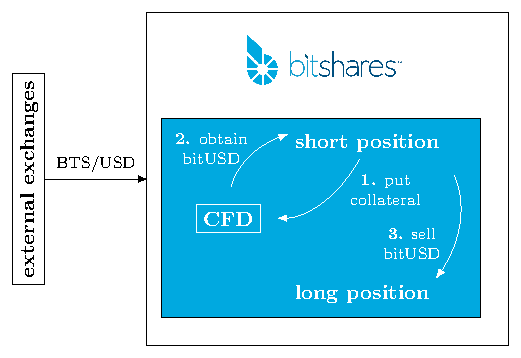
\includegraphics[width=.8\linewidth]{figures/external-pricefeed}
 \end{center}
 \caption{Illustration of external price discovery and a ``short sell'' to seek
          greater exposure for BTS price movements.}
 \label{fig:btsdex}
\end{figure}

The collateral is only returned to the short seller when the corresponding
amount of the asset agreed in the contract is handed over to the BitShares
network again. The protocol will then effectively destroy these tokens and
fulfill the contract. This is referred to as \emph{covering a
short}. At the moment of creation, the position of the \emph{shorter} has not
changed at all because he can directly cover his own short position using the
bitUSD to gain back his BTS used as collateral.

If the short seller has sold the SmartCoins he has created, then he would be
required to purchase them back from the market before closing his short
position. Meanwhile, if the value of the collateral relative to the current price
of the market pegged asset falls below a certain margin of safety, the assets
can be automatically (i.e. initiated by the protocol itself) repurchased from
the market before the collateral becomes insufficient.

These rules create systemic demand for market pegged assets while allowing them
to remain fungible. To protect your contract against \emph{margin calls}
(automated, network initiated force settlement of your contract at the price
feed), you should at least maintain the so called \emph{maintenance collateral
level} at all times. Hence, the collateral only needs to be high enough to
cover any slippage as a result of a short squeeze.

In summary, the following set of market rules apply to all market pegged assets
(for the sake of simplicity, we here focus on the MPA bitUSD):
\begin{itemize}
 \item Anyone with BitUSD can settle their position within an
       interval\footnote{defined by the shareholder approval} at the settlement
       price (identical to the feed price).
 \item In this case, the \emph{least} collateralized short positions would be
       margin called and their collateral would be used to settle the position.
 \item The price feed is the median of many sources that are updated at least
       once per hour.
 \item Short positions never expire, except by hitting the maintenance
       collateral limit, or being force-settled as the least collateralized at the
       time of forced settlement (see point 2).
 \item In the event that the least-collateralized short position lacks enough
       collateral to cover at the price feed, then all BitUSD positions are
       automatically force settled at the price of the least collateralized
       short (black swan event, see~\cref{sec:blackswan}).
\end{itemize}

These simple rules enable a price floor of \$1.00 for 1.00 BitUSD. A simple
metric for testing the validity of our claim is to demonstrate that, if you can
find someone willing to sell 1.00 BitUSD for \$1.00, that it would be the
cheapest option for buying BTS. This means that 100\% of the buying demand for
BTS would be available to give liquidity to BitUSD holders as a priority over
BTS holders.
